% Chapter 18 -- Claim: High-Interest Currencies Depreciate Enough to Offset Their Yield
% Requires: amsmath, amssymb, booktabs, array, tabularx, graphicx, tcolorbox (breakable, skins), hyperref or url.
% Defines the callout box only if the preamble has not.
\providecolor{fenavy}{HTML}{1B2A6B}
\providecolor{feshade}{HTML}{F3F5FA}
\makeatletter
\@ifundefined{callout}{%
  \newtcolorbox{callout}{breakable, enhanced,
    colback=white, colframe=gray!70, boxrule=0.5pt, arc=1mm,
    borderline west={2.5pt}{0pt}{gray!70},
    left=8pt, right=8pt, top=4pt, bottom=4pt}%
}{}
\makeatother

\chapter{Claim: High-Interest Currencies Depreciate Enough to Offset Their Yield}
\label{ch:18}

In 2007 a Japanese household could borrow yen at less than 1\% and deposit Australian dollars at more than 6\%. Japanese retail investors, nicknamed ``Mrs.\ Watanabe,'' and hedge funds did this on a large scale. If exchange rates had stayed put, the trade would have earned the difference, year after year.

Textbook theory says it should not work. If investors are risk-neutral and rational, a currency that pays a higher interest rate must be expected to fall by just enough to offset its yield advantage. Otherwise everyone would borrow in yen and lend in Australian dollars until the opportunity disappeared. This is \textbf{uncovered interest parity}, and it underpins much of international macroeconomics.

This chapter tests it, and it turns out to be one of the most persistent puzzles in finance. The test also shows what the carry trade's returns look like and how they end.

By the end of the chapter you will be able to:

\begin{itemize}
  \item quote exchange rates and measure currency returns in logs;
  \item compute a forward exchange rate from covered interest parity, and explain why arbitrage enforces it;
  \item state uncovered interest parity and compute the profit or loss on a carry trade;
  \item run and interpret the Fama regression, and explain the forward premium puzzle;
  \item compare the risk-premium, crash-risk and slow-adjustment explanations, and the evidence for each;
  \item judge what a currency carry fund is paid for and how it loses money.
\end{itemize}

\section{Foundations: exchange rates, forwards and interest parity}
\label{sec:18-foundations}

\textbf{Exchange rates.} The \textbf{spot rate} $S$ is the price of one currency in terms of another. In this chapter $S$ is the number of U.S. dollars per unit of foreign currency, so a rise in $S$ means the foreign currency has \textbf{appreciated}. Changes are measured in logs: $\Delta s_{t+1} = \ln(S_{t+1}/S_t)$.

\textbf{Forward rates and covered interest parity (CIP).} A forward contract fixes today the exchange rate $F$ for a trade at a future date. An investor can earn the dollar interest rate $i$ either directly, or by converting dollars to foreign currency, earning the foreign rate $i^*$, and converting back at the forward rate. Arbitrage makes the two equal:
\begin{equation}
  \frac{F}{S} = \frac{1 + i}{1 + i^*}, \qquad \text{or in logs,} \qquad f - s \approx i - i^*
  \label{eq:18-cip}
\end{equation}
The forward rate is below the spot rate for a high-interest currency: the \textbf{forward discount} equals the interest differential. CIP held closely until 2008 and has shown small but persistent deviations since (Du, Tepper and Verdelhan 2018).

\textbf{Uncovered interest parity (UIP)} goes further. It says the \emph{expected} future spot rate equals the forward rate, so the high-interest currency is expected to depreciate by the interest differential:
\begin{equation}
  E_t[\Delta s_{t+1}] = i_t - i^*_t
  \label{eq:18-uip}
\end{equation}
UIP has no arbitrage behind it. Holding a foreign currency unhedged is risky, so UIP holds only if investors require no premium for that risk.

\textbf{The carry trade.} Borrow in a low-interest currency, convert and invest in a high-interest currency, and convert back later without hedging. Its excess return is the interest differential plus the change in the exchange rate:
\begin{equation}
  rx_{t+1} = (i^*_t - i_t) + \Delta s_{t+1}
  \label{eq:18-carry}
\end{equation}
Under UIP its expected value is zero. Equivalently, the carry trade is buying high-interest currencies forward at a discount and hoping they do not fall by as much as the discount.

\textbf{Worked example.} The U.S. one-year rate is 1\%, the Australian rate 5\%, and the spot rate is \$0.70 per Australian dollar (Figure~\ref{fig:18-carry}).

\begin{itemize}
  \item CIP: the one-year forward rate is $0.70 \times 1.01/1.05 \approx \$0.673$.
  \item UIP: the expected spot rate in a year is also \$0.673, a 3.8\% depreciation.
  \item Carry trade: borrow \$1 million at 1\%, buy A\$1.429 million, invest at 5\% to get A\$1.5 million.
  \begin{itemize}
    \item Spot unchanged at \$0.70: proceeds \$1.05 million, repay \$1.01 million, profit \$40,000.
    \item Spot falls to \$0.673, as UIP predicts: proceeds \$1.01 million, profit zero.
    \item Spot falls 10\% to \$0.63: proceeds \$945,000, loss \$65,000.
  \end{itemize}
\end{itemize}

\begin{figure}[htbp]
\centering
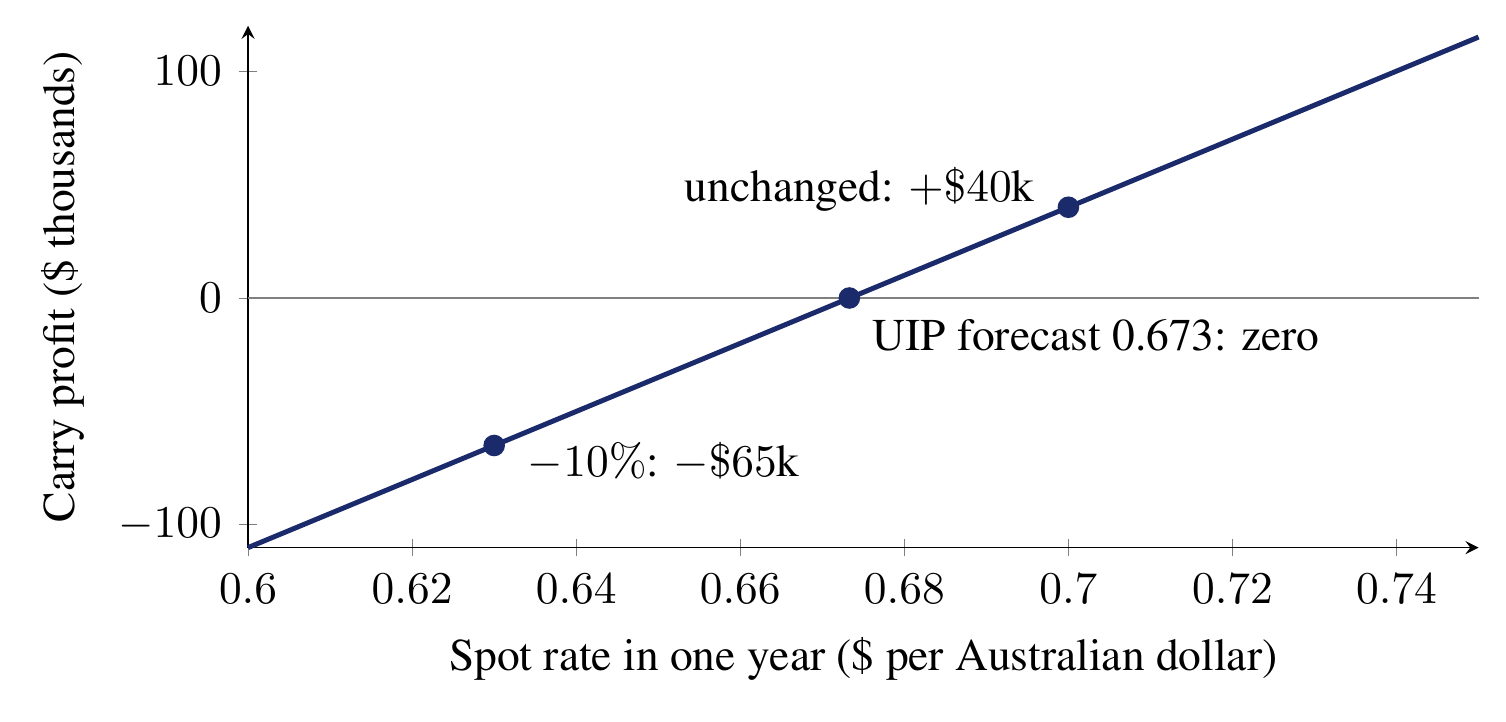
\includegraphics[width=0.85\linewidth]{images/fig18-1-carry-payoff.png}
\caption{Profit on the worked example's carry trade against the spot rate a year later. The trade earns \$40,000 if the Australian dollar is unchanged, breaks even at the UIP forecast of \$0.673, and loses \$65,000 if the currency falls 10\%.}
\label{fig:18-carry}
\end{figure}

\textbf{Further reading.} Hull, \emph{Options, Futures, and Other Derivatives} (foreign exchange forwards and futures, interest rate parity); Krugman, Obstfeld and Melitz, \emph{International Economics: Theory and Policy} (interest parity and exchange rate determination); Bodie, Kane and Marcus, \emph{Investments} (international diversification and currency risk); Cochrane, \emph{Asset Pricing} (the forward premium puzzle).

\section{How it works}
\label{sec:18-how}

UIP can be tested in two ways, one for each currency and one across currencies.

\textbf{The Fama regression.} Regress the change in the exchange rate on the lagged interest differential:
\begin{equation}
  \Delta s_{t+1} = a + b\,(i_t - i^*_t) + e_{t+1}
  \label{eq:18-fama}
\end{equation}
UIP implies $b = 1$: a one-point interest advantage for the foreign currency predicts a one-point depreciation. If $b = 0$, exchange rates are a random walk and the carry trade earns the whole differential. If $b < 0$, high-interest currencies tend to \emph{appreciate}, and the carry trade earns more than the differential (Figure~\ref{fig:18-fama}). This is the \textbf{forward premium puzzle}.

\begin{figure}[htbp]
\centering
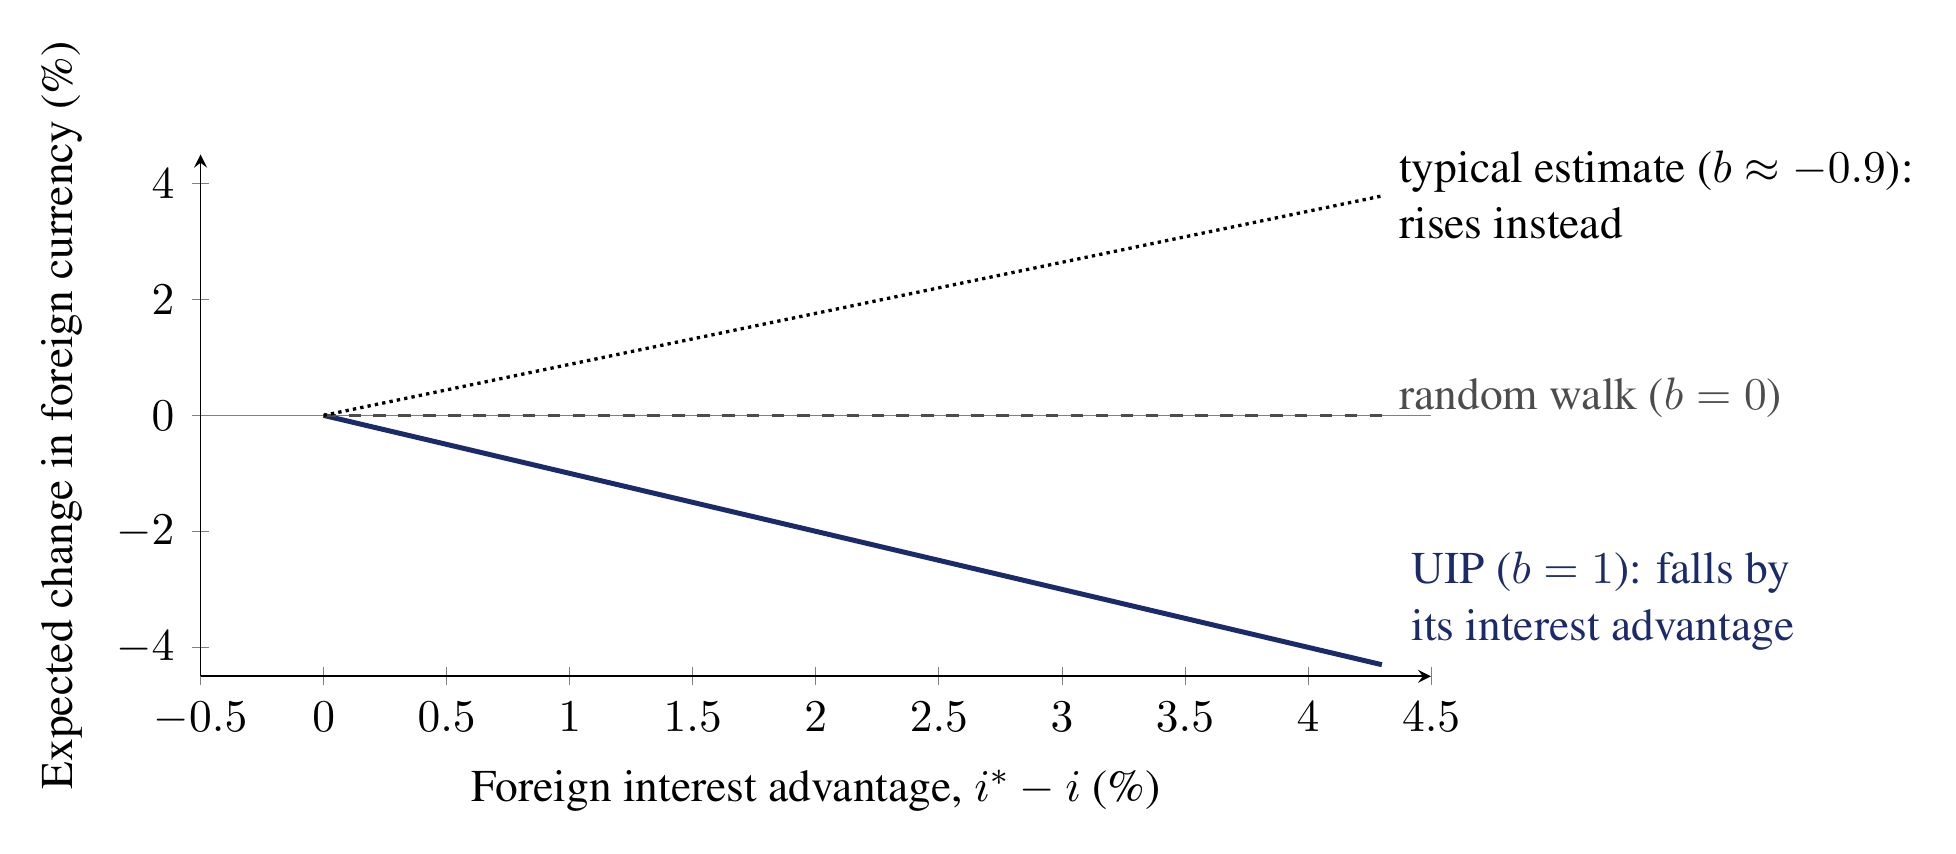
\includegraphics[width=0.85\linewidth]{images/fig18-2-fama-slope.png}
\caption{Three readings of the Fama regression. Under UIP ($b = 1$), a currency with a higher interest rate falls by its interest advantage. Under a random walk ($b = 0$), it is expected not to move. The typical estimate ($b \approx -0.9$, Froot and Thaler 1990) implies that it rises instead.}
\label{fig:18-fama}
\end{figure}

\textbf{Carry portfolios.} Each month, sort currencies by their interest rate, buy the highest-yielding ones and sell the lowest. If UIP holds, the portfolio earns nothing on average. Portfolios diversify away currency-specific noise and are what investors actually trade.

\textbf{Why UIP might fail.} There are three broad explanations.

\begin{itemize}
  \item \textbf{A risk premium.} High-interest currencies tend to fall in global downturns, when investors flee to the dollar, yen and Swiss franc. Investors demand a premium for holding them. Lustig, Roussanov and Verdelhan (2011) argue that carry returns compensate for exposure to a global risk factor.
  \item \textbf{Crash risk.} Carry returns may be steady most of the time and then collapse when carry traders all unwind at once, as funding dries up. The premium pays for those crashes (Brunnermeier, Nagel and Pedersen 2008).
  \item \textbf{Slow adjustment.} Investors may underreact to interest-rate changes, so currencies move toward UIP only gradually. That would be a mispricing rather than a risk premium, and should shrink as more capital pursues it.
\end{itemize}

These explanations make different predictions. A risk premium should show up as losses in bad times for the world economy. Crash risk should show up as negative skewness and losses concentrated in a few episodes. Slow adjustment should show up as a premium that declines over time and does not depend on market conditions.

\section{The claim}
\label{sec:18-claim}

\begin{callout}
\textbf{Claim (uncovered interest parity).} The currency of a high-interest country is expected to depreciate by its interest advantage, so borrowing in low-interest currencies and lending in high-interest ones earns nothing on average.
\end{callout}

To test it we need to be precise on three points.

\begin{itemize}
  \item \textbf{On average, over what period.} UIP is a statement about expectations. Over a few months, exchange-rate noise dominates. The test needs decades of data and many currencies.
  \item \textbf{Which currencies.} The lab uses nine developed-market currencies against the dollar. Emerging-market currencies have higher carry but also capital controls, default risk and much higher trading costs.
  \item \textbf{What would count against it.} UIP fails if Fama slopes are significantly below 1 and if a carry portfolio earns a significant average return. It fails in a deeper sense if the return survives trading costs and the slopes are below zero, not merely below one.
\end{itemize}

\section{The original evidence}
\label{sec:18-evidence}

\textbf{Fama (1984).} Using monthly data for nine currencies against the dollar after the end of fixed exchange rates in 1973, Fama found that the slopes were not just below 1 but generally negative. High-interest currencies tended to appreciate. He showed that this implies a risk premium in forward rates that varies over time and is more volatile than expected exchange-rate changes. Froot and Thaler (1990) summarized the literature: across 75 published estimates, the average slope was about $-0.88$.

\textbf{Carry as a risk factor.} Lustig, Roussanov and Verdelhan (2011) sorted currencies into portfolios by interest rate. The high-minus-low portfolio earned substantial average returns. They showed that a single carry factor, together with a dollar factor, explained much of the cross-section of currency returns, and that high-interest currencies loaded more heavily on it. Menkhoff, Sarno, Schmeling and Schrimpf (2012) found that carry losses coincided with increases in global currency volatility.

\textbf{Crashes.} Brunnermeier, Nagel and Pedersen (2008) showed that carry returns are negatively skewed: large losses are more likely than large gains. Losses coincided with falling risk appetite and funding liquidity, measured among other things by rises in the VIX, as carry traders were forced to unwind together.

\textbf{Peso problems.} One possible explanation is that the high returns compensate for rare disasters not yet seen in the sample, a \textbf{peso problem}. Burnside, Eichenbaum, Kleshchelski and Rebelo (2011) tested this by hedging carry positions with currency options. The hedged trade still earned a substantial return. They concluded that rare disasters could explain the premium only if the market prices them at much more than their likely cost.

\section{Replication lab: G10 currencies against the dollar}
\label{sec:18-lab}

\begin{callout}
\textbf{Lab 18 at a glance.} \emph{Claim on trial:} high-interest currencies depreciate enough to offset their yield. \emph{Data:} free monthly data from FRED: the Federal Reserve's exchange rates for nine currencies (yen, pound, Swiss franc, Canadian, Australian and New Zealand dollars, Swedish krona and Norwegian krone, and the euro from 1999) and OECD three-month interbank rates for each country and the United States. The VIX and the Fama--French market factor are optional. \emph{Code:} runs as a script (\texttt{python lab18.py}) or as a notebook with a prediction prompt before each step.
\end{callout}

\textbf{Part A, Fama regressions.} For each currency, the monthly change in the log exchange rate (dollars per foreign unit) on last month's U.S.-minus-foreign interest differential, with Newey--West errors, plus a pooled slope (Figure 18.3).

\textbf{Part B, the carry portfolio.} Each month, long the three highest-rate currencies and short the three lowest, equally weighted, using rates known at the end of the previous month. The return is split into the interest earned and the exchange-rate change (Figure 18.4). Its distribution is compared with a normal distribution (Figure 18.5).

\textbf{Part C, stress tests.} Three subperiods (to 1998, 1999--2007, 2008 onward), transaction costs of 0 to 20 basis points per unit of weight traded, exposure to stock-market returns and to changes in the VIX, and the ten worst months.

\textbf{Part D, the investor's view.} Drawdowns, recovery times, the share of losses from the worst months, and carry returns plotted against VIX changes (Figures 18.6 and 18.7).

Three data choices matter.

\begin{itemize}
  \item The interest differential stands in for the forward discount, which covered interest parity makes nearly equal; forward rates are not freely available.
  \item FRED's exchange rates are monthly averages of daily rates, which smooths returns and makes crashes look milder than they were.
  \item The sample is limited to developed currencies, where carry is smaller but trading costs and capital controls are minor.
\end{itemize}

\textbf{What the simulated run shows.} The simulation lets high-rate currencies depreciate by only 30\% of their interest advantage and adds rare risk-off months in which they fall sharply. The lab recovers this: a pooled Fama slope well below 1, a carry portfolio with a positive average return and negative skewness, interest income partly offset by exchange-rate losses, and losses when the VIX jumps. Individual currency slopes are very imprecise, as they are in real data. These results confirm that the code works. They say nothing about real markets. Run the lab on the real data to reach your own verdict.

\section{Stress tests}
\label{sec:18-stress}

\textbf{Subperiods.} Carry returns have varied a lot over time. A strategy that earns most of its return in a few long calm stretches and gives back much of it in a few months can look very different depending on where the sample starts and ends. The period since 2008 matters most: interest-rate differentials among developed countries collapsed toward zero for years, and with them the carry available.

\textbf{Transaction costs.} G10 currencies are the most liquid assets in the world, with bid--ask spreads of a few basis points. Carry portfolios rebalance only when interest rankings change, so turnover is modest. Costs reduce but rarely eliminate the developed-market carry premium. For emerging-market currencies they matter much more.

\textbf{Skewness and crashes.} The carry trade is often described as ``going up the stairs and down the elevator.'' Its returns should show negative skewness, and its worst months should cluster in episodes of global stress: 1992 (the European exchange-rate crisis), 1998 (the Russian default and LTCM), 2008, and the yen rally of August 2024. The lab lists the worst months and their share of total losses.

\textbf{Exposure to stocks and fear.} If carry is a risk premium, its returns should be positively correlated with stock returns, especially in bad months, and negatively correlated with changes in the VIX. A strategy whose beta to stocks rises in down markets offers less diversification than its average correlation suggests.

\textbf{Monthly averages.} Because the exchange rates are monthly averages of daily data, the lab's worst months will understate the speed of the real crashes. In October 2008 several carry currencies fell by double digits against the yen within days.

\section{Verdict}
\label{sec:18-verdict}

\begin{callout}
\textbf{Verdict: fails} (as of October 2026) over most samples. High-interest currencies have not depreciated by their interest advantage on average; Fama slopes are well below 1 and often negative, and carry portfolios have earned a premium. That premium is paid for with sudden crashes that arrive in global downturns.
\end{callout}

What fails:

\begin{itemize}
  \item \textbf{The slope.} Across decades of studies, slopes in the Fama regression have been below 1 and usually below zero. A high interest rate has predicted, if anything, a stronger currency in the short run.
  \item \textbf{The zero-return prediction.} Carry portfolios have earned positive average returns after realistic costs for developed-market currencies.
\end{itemize}

What survives:

\begin{itemize}
  \item \textbf{The spirit of UIP over long horizons and in extremes.} Some studies find slopes closer to 1 at horizons of several years, and in countries with very high inflation, where large interest differentials are matched by large depreciations.
  \item \textbf{No free lunch.} The premium comes with negative skewness, losses concentrated in global crises and positive correlation with stocks in bad months. That is what a risk premium looks like, not an arbitrage. An investor who earns carry is paid for providing liquidity and insurance to the rest of the world when it is scarce.
\end{itemize}

The verdict would move to \emph{weakens} if carry returns since 2008 were consistently near zero, as narrow interest differentials and crowding might imply.

\section{What investors can use}
\label{sec:18-investors}

\textbf{What a currency carry fund earns.} A carry strategy collects interest-rate differentials between currencies and keeps them as long as exchange rates do not move against it. In calm years it delivers modest, steady gains. Its risk is not spread evenly over time: most of its losses come in a few months of global stress, when high-yielding currencies fall together and funding currencies, the yen and Swiss franc above all, rise.

\textbf{How it loses money.} Carry crashes are fast. They begin when something forces leveraged carry traders to cut positions: a rise in volatility, a margin call, a surprise from the central bank of a funding currency. Selling pushes high-yield currencies down further, which forces more selling. Diversifying across many currency pairs helps little, because the losses are driven by a common factor.

\textbf{Carry in a portfolio.} Because carry tends to lose when stocks fall, it adds less diversification to an equity portfolio than its average correlation suggests. Investors should measure its correlation with stocks in bad months, not over the whole sample.

\textbf{Questions to ask a manager running currency carry:}

\begin{itemize}
  \item What are the funding currencies, and how concentrated is the portfolio in one or two pairs?
  \item How much leverage is used, and what happens to margin in a volatility spike?
  \item How did the strategy perform in late 2008 and in August 2024?
  \item Is there a crash filter, such as cutting exposure when volatility rises, and how did it perform out of sample?
\end{itemize}

\begin{callout}
\textbf{What Failed: the yen carry trade, 2008.} In the years before 2008, borrowing in yen at rates near zero and investing in Australian dollars, New Zealand dollars and other high-yielding currencies was one of the most popular trades in the world, among Japanese retail investors and hedge funds alike. When the financial crisis intensified in the autumn of 2008, carry traders rushed to repay yen loans at the same time. Between July and late October 2008 the Australian and New Zealand dollars lost more than a third of their value against the yen, wiping out years of interest income in a few weeks.

The episode matched the risk-premium explanation exactly. The trade paid steadily in good times and lost heavily in the worst global downturn in decades, when investors could least afford it. It recurred on a smaller scale in August 2024: after the Bank of Japan raised its policy rate to 0.25\% at the end of July, the yen rose sharply, carry positions were cut, and on August 5 the Nikkei 225 fell 12.4\%.
\end{callout}

\section{Open questions}
\label{sec:18-open}

\begin{itemize}
  \item \textbf{Is carry a risk premium or a slowly corrected mispricing?} If it were mispricing, it should shrink as more capital pursues it. Has it?
  \item \textbf{What happened to carry after 2008?} Near-zero rates in many developed countries removed most interest differentials. Did the premium per unit of differential change, or only the opportunity?
  \item \textbf{Do covered-interest-parity deviations matter?} Since 2008, CIP has not held exactly, reflecting the cost of banks' balance sheets. How does this affect measured carry returns?
  \item \textbf{Can crashes be avoided?} Momentum and volatility filters claim to sidestep the worst months. Do they work out of sample, or do they simply give up the premium?
\end{itemize}

\section*{Exercises}
\addcontentsline{toc}{section}{Exercises}

\subsection*{Conceptual (all readers)}

\begin{enumerate}
  \item The U.S. one-year rate is 4\% and the Japanese rate 0.5\%. The spot rate is 150 yen per dollar. Compute the one-year forward rate. Under UIP, what spot rate is expected in a year?
  \item Using the numbers in Exercise 1, compute the return to a dollar-based investor who borrows yen, converts to dollars and invests at 4\%, if the spot rate stays at 150, moves to the UIP forecast, or falls to 135.
  \item Explain why covered interest parity is enforced by arbitrage but uncovered interest parity is not.
\end{enumerate}

\subsection*{Lab extensions (technical readers)}

\begin{enumerate}
  \setcounter{enumi}{3}
  \item Part A: how many currencies have Fama slopes significantly below 1? Below 0? What is the pooled slope?
  \item Part B: what share of the carry portfolio's interest income was offset by exchange-rate changes? Compare with what UIP predicts.
  \item Part C: compare carry returns before and after 2008. What happened to the interest differentials?
  \item Part C: estimate the carry portfolio's beta to stocks in all months and in months when stocks fell. What does the difference mean for an investor?
  \item Add a filter that holds the carry portfolio only when the VIX is below its 12-month median. Compare the Sharpe ratio and the worst month with the unfiltered strategy.
  \item A financial adviser recommends a fund that earns ``the interest-rate differential between currencies.'' Using this chapter's evidence, explain what the fund is really paid for and when it is likely to lose money.
\end{enumerate}

\section*{References}
\addcontentsline{toc}{section}{References}

\begin{itemize}
  \item Brunnermeier, M. K., Nagel, S. and Pedersen, L. H. (2008). Carry Trades and Currency Crashes. \emph{NBER Macroeconomics Annual} 23: 313--347.
  \item Burnside, C., Eichenbaum, M., Kleshchelski, I. and Rebelo, S. (2011). Do Peso Problems Explain the Returns to the Carry Trade? \emph{Review of Financial Studies} 24(3): 853--891.
  \item Du, W., Tepper, A. and Verdelhan, A. (2018). Deviations from Covered Interest Rate Parity. \emph{Journal of Finance} 73(3): 915--957.
  \item Fama, E. F. (1984). Forward and Spot Exchange Rates. \emph{Journal of Monetary Economics} 14(3): 319--338.
  \item Froot, K. A. and Thaler, R. H. (1990). Anomalies: Foreign Exchange. \emph{Journal of Economic Perspectives} 4(3): 179--192.
  \item Lustig, H., Roussanov, N. and Verdelhan, A. (2011). Common Risk Factors in Currency Markets. \emph{Review of Financial Studies} 24(11): 3731--3777.
  \item Menkhoff, L., Sarno, L., Schmeling, M. and Schrimpf, A. (2012). Carry Trades and Global Foreign Exchange Volatility. \emph{Journal of Finance} 67(2): 681--718.
\end{itemize}

\textbf{Data:} Board of Governors of the Federal Reserve System, H.10 exchange rates; OECD, Main Economic Indicators, three-month interbank rates; retrieved from FRED, Federal Reserve Bank of St.\ Louis. Optional: CBOE Volatility Index [VIXCLS], FRED; Kenneth R. French Data Library.
